\documentclass[11pt,a4paper]{article}

\usepackage[T1]{fontenc}
\usepackage[brazilian]{babel}
\usepackage{lmodern}
\usepackage[margin=2.5cm]{geometry}
\usepackage{graphicx}
\usepackage{subcaption}
\usepackage{float}
\usepackage{booktabs}
\usepackage{array}
\usepackage{xcolor}
\usepackage{listings}
\usepackage[hidelinks]{hyperref}
\Urlmuskip=0mu plus 1mu\relax   % permite quebrar URLs longas no fim da linha
\emergencystretch=3em

\newcommand{\autor}{Rafael Sardinha}
\newcommand{\disciplina}{Desenvolvimento Web II}
\newcommand{\linkrepo}{\url{https://github.com/rafaelsardinhadev/DWEB2/tree/master/pubsub-php}}

\lstset{
  basicstyle=\ttfamily\fontsize{6.3}{7.6}\selectfont,
  breaklines=true,
  breakindent=0pt,
  columns=fullflexible,
  keepspaces=true,
  frame=single,
  rulecolor=\color{black!30},
  backgroundcolor=\color{black!3},
  xleftmargin=0pt,
  aboveskip=6pt,
  belowskip=6pt
}

\newfloat{logfloat}{htbp}{lol}
\floatname{logfloat}{Log}
\newcommand{\logfig}[3]{\begin{logfloat}[htbp]\lstinputlisting{#1}\caption{#2}\label{#3}\end{logfloat}}
\captionsetup{font=small,labelfont=bf}

\makeatletter
\setlength{\@fptop}{0pt}
\setlength{\@fpsep}{14pt}
\setlength{\@fpbot}{0pt plus 1fil}
\makeatother

\title{Laborat\'orio de Publish/Subscribe com ActiveMQ\\[2pt]
\large Implementa\c{c}\~ao em PHP com STOMP}
\author{\autor\\ \disciplina}
\date{\today}

\begin{document}
\maketitle

\begin{abstract}
Este trabalho implementa e testa o modelo \textit{publish/subscribe} em PHP, sobre o
\textit{broker} Apache ActiveMQ executado em Docker e com STOMP. Um
publicador envia cinco mensagens com intervalo de um minuto e cinco inst\^ancias de
assinante leem uma mensagem cada. Foram explorados fan-out (t\'opico), fila, mensagens
persistentes e assinaturas dur\'aveis.
\end{abstract}

\section{Introdu\c{c}\~ao}

O objetivo \'e praticar o modelo de publica\c{c}\~ao e assinatura com um
\textit{broker} de mensagens. Os requisitos foram: usar o ActiveMQ com Docker; criar um
programa cliente que publique cinco mensagens com um minuto de intervalo entre elas;
criar o programa que leia as mensagens, com cinco inst\^ancias que leem uma vez cada; e
explorar as op\c{c}\~oes de envio (fan-out, persist\^encia, entre outras).

A solu\c{c}\~ao foi feita em PHP, com a biblioteca \texttt{stomp-php}, e inclui uma
p\'agina web para operar os programas pelo navegador. O c\'odigo-fonte est\'a em \linkrepo.

\section{Referencial te\'orico}

\subsection{Publish/subscribe}
No modelo \textit{publish/subscribe}, quem produz a mensagem (publicador) n\~ao
conhece quem a consome (assinante). Isso desacopla os dois lados de tr\^es formas: no
\emph{espa\c{c}o} (os participantes n\~ao se conhecem), no \emph{tempo} (n\~ao precisam estar
ativos ao mesmo tempo) e na \emph{sincroniza\c{c}\~ao} (o envio e o recebimento n\~ao
bloqueiam um ao outro). Esse papel de intermedi\'ario \'e exercido pelo \textit{broker},
que recebe, guarda e entrega as mensagens.

\subsection{T\'opicos e filas}
Os v\'ideos indicados na atividade~\cite{savoir,redblack} tratam da diferen\c{c}a entre
filas e t\'opicos. Em resumo, o \textit{broker} oferece dois tipos de destino:

\begin{itemize}
  \item \textbf{T\'opico (fan-out):} cada assinante ativo recebe uma c\'opia de cada
        mensagem. Serve para difundir um evento a v\'arios interessados.
  \item \textbf{Fila (consumidores concorrentes):} cada mensagem \'e entregue a
        \emph{um} s\'o consumidor. Serve para dividir trabalho entre inst\^ancias.
\end{itemize}

\subsection{Persist\^encia e durabilidade}
S\~ao dois conceitos diferentes. A \textbf{persist\^encia} \'e uma propriedade da
\emph{mensagem}: se for persistente, o \textit{broker} a grava em disco e ela sobrevive a uma reinicializa\c{c}\~ao; se n\~ao for,
fica s\'o na mem\'oria. A \textbf{durabilidade} \'e uma propriedade da \emph{assinatura}
de um t\'opico: com uma assinatura dur\'avel, o \textit{broker} guarda as mensagens
enquanto o assinante est\'a desligado e as entrega quando ele volta. Sem ela, o
assinante que estava offline perde o que foi publicado nesse intervalo.

\subsection{STOMP e ActiveMQ}
O \textbf{STOMP} (\textit{Simple Text Oriented Messaging Protocol}) \'e um
protocolo simples, baseado em texto, com comandos como \texttt{CONNECT},
\texttt{SEND}, \texttt{SUBSCRIBE}, \texttt{ACK} e \texttt{UNSUBSCRIBE}. O \textbf{Apache
ActiveMQ Classic} aceita STOMP em uma porta pr\'opria e oferece
extens\~oes por cabe\c{c}alhos, usadas aqui para assinaturas dur\'aveis e controle de
entrega. No PHP, a conex\~ao \'e feita pela biblioteca \texttt{stomp-php}.

\section{Implementa\c{c}\~ao}

\subsection{Ambiente}
O ActiveMQ Classic 6.2.0 roda com Docker. O sistema foi desenvolvido com PHP 8.4,
Composer e \texttt{stomp-php} 5.1.4, e testado no Windows 11.

\subsection{Programas de linha de comando}
\begin{itemize}
  \item \texttt{publicador.php}: publica uma quantidade de mensagens em um t\'opico ou
        fila, esperando um intervalo entre elas. Aceita
        o destino, o nome, o modo de entrega (persistente ou n\~ao), a quantidade e o
        intervalo.
  \item \texttt{assinante.php}: l\^e mensagens de um t\'opico ou fila e encerra (padr\~ao: uma
        mensagem por inst\^ancia, \emph{``l\^e uma vez''}). Aceita o n\'umero da inst\^ancia,
        o destino, a assinatura dur\'avel e a quantidade de mensagens a ler. Cinco
        inst\^ancias s\~ao cinco processos independentes, cada um com seu \texttt{--id}.
\end{itemize}
Cada linha de log traz o hor\'ario e a inst\^ancia, o que permite acompanhar a ordem dos
eventos.

\subsection{P\'agina web}
A p\'agina permite escolher o destino (t\'opico ou fila), iniciar os assinantes e
publicar as mensagens, mostrando o que cada assinante recebeu. Uma requisi\c{c}\~ao web dura
s\'o um instante, mas um assinante precisa ficar vivo esperando mensagens. Por isso o
\texttt{api.php} inicia o \texttt{assinante.php} e o \texttt{publicador.php} como
processos em segundo plano, que gravam o andamento em arquivos JSON; a p\'agina consulta
o estado a cada segundo. O bot\~ao \emph{Desconectar} deixa um assinante offline e o
\emph{Conectar} o liga de novo, o que permite testar o comportamento da assinatura
dur\'avel. Para o visual da p\'agina foi usada uma biblioteca de CSS pronta (Sakura).

\subsection{Recursos do STOMP usados}
\begin{table}[H]
\centering
\small
\begin{tabular}{@{}>{\raggedright\arraybackslash}p{5cm}>{\raggedright\arraybackslash}p{9.6cm}@{}}
\toprule
\textbf{Recurso} & \textbf{Como foi usado} \\
\midrule
T\'opico e fila         & destinos \texttt{/topic/nome} e \texttt{/queue/nome} \\
Mensagem persistente   & cabe\c{c}alho \texttt{persistent:true} no \texttt{SEND} \\
Assinatura dur\'avel    & \texttt{client-id} no \texttt{CONNECT} e cabe\c{c}alho \texttt{activemq.subscriptionName} no \texttt{SUBSCRIBE} \\
Confirma\c{c}\~ao        & modo \texttt{client-individual}: a mensagem s\'o sai do \textit{broker} depois do \texttt{ACK} \\
Uma mensagem por vez   & cabe\c{c}alho \texttt{activemq.prefetchSize:1}, que divide a fila entre os assinantes \\
Remover assinatura     & desligar o consumidor e enviar \texttt{UNSUBSCRIBE} com o nome da assinatura \\
\bottomrule
\end{tabular}
\caption{Recursos do STOMP e das extens\~oes do ActiveMQ usados no laborat\'orio.}
\end{table}

\section{Resultados}

\subsection{Metodologia}
Cada cen\'ario foi executado pelo terminal e pela p\'agina web. A rodada completa do
enunciado, com cinco mensagens a cada 60 s (cerca de 4 minutos), foi feita no terminal
(fan-out) e na p\'agina (fila). Nos demais testes, e nos prints da p\'agina, o intervalo foi
reduzido a 1--2 s s\'o para agilizar, pois o resultado n\~ao depende dele.

\subsection{Cen\'ario 1: fan-out (t\'opico)}
Cinco assinantes de um t\'opico foram ligados antes do envio. Todos receberam a
mesma mensagem 1/5, e o publicador continuou enviando uma mensagem por minuto
(Figura~\ref{fig:fanout} e Log~\ref{log:fan}).

\begin{figure}[htbp]
\centering
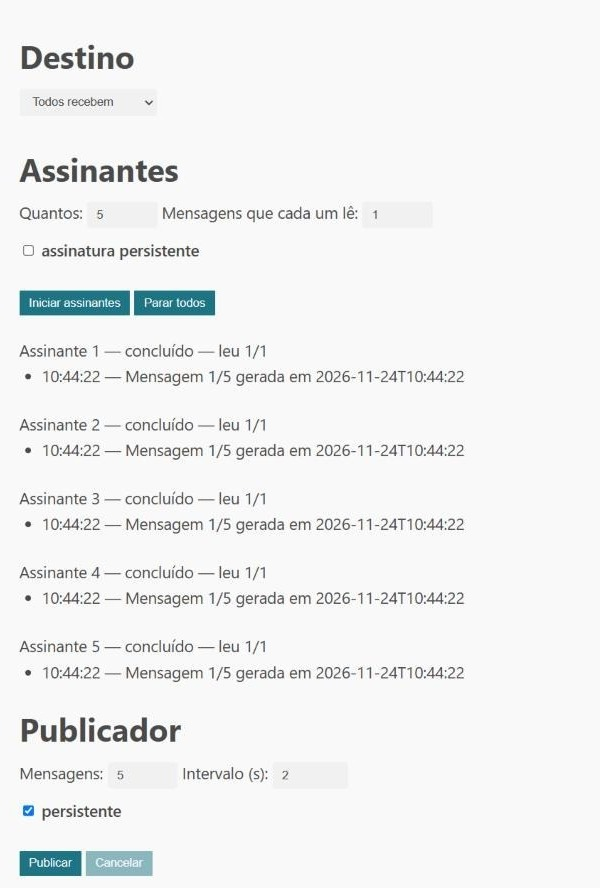
\includegraphics[width=0.5\textwidth]{figuras/php-fanout.jpg}
\caption{Fan-out na p\'agina web: os cinco assinantes receberam a mensagem 1/5.}
\label{fig:fanout}
\end{figure}

\logfig{logs/php-terminal-60s-fanout.txt}{Fan-out no terminal, rodada de 60 s: o publicador envia a cada minuto e os cinco assinantes recebem a mensagem 1.}{log:fan}

\subsection{Cen\'ario 2: fila}
Com cinco consumidores na mesma fila, cada mensagem foi entregue a um \'unico
assinante, e cada assinante recebeu uma mensagem diferente (Figura~\ref{fig:filand}a e
Log~\ref{log:fila}).

\logfig{logs/php-terminal-fila.txt}{Fila no terminal: cada mensagem vai para um assinante.}{log:fila}

\subsection{Cen\'arios 3 e 4: assinante offline}
O Assinante~3 foi desconectado antes do envio e reconectado depois. No t\'opico
\emph{n\~ao dur\'avel} ele n\~ao recebeu nenhuma das tr\^es mensagens
(Figura~\ref{fig:filand}b); com a assinatura \emph{dur\'avel} recebeu as tr\^es ao voltar
(Figura~\ref{fig:dur}). Os Logs~\ref{log:nd} e~\ref{log:dur} mostram o mesmo roteiro no
terminal; no segundo, a assinatura \'e removida do \textit{broker} no final.

\begin{figure}[htbp]
\centering
\begin{subfigure}[t]{0.40\textwidth}
  \centering
  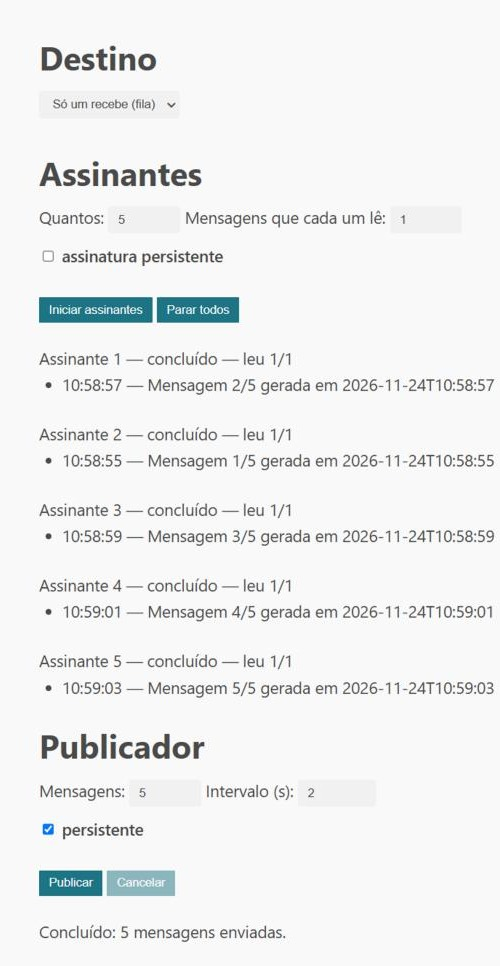
\includegraphics[width=\textwidth]{figuras/php-fila.jpg}
  \caption{Fila: cada assinante recebeu uma mensagem diferente.}
\end{subfigure}\hfill
\begin{subfigure}[t]{0.40\textwidth}
  \centering
  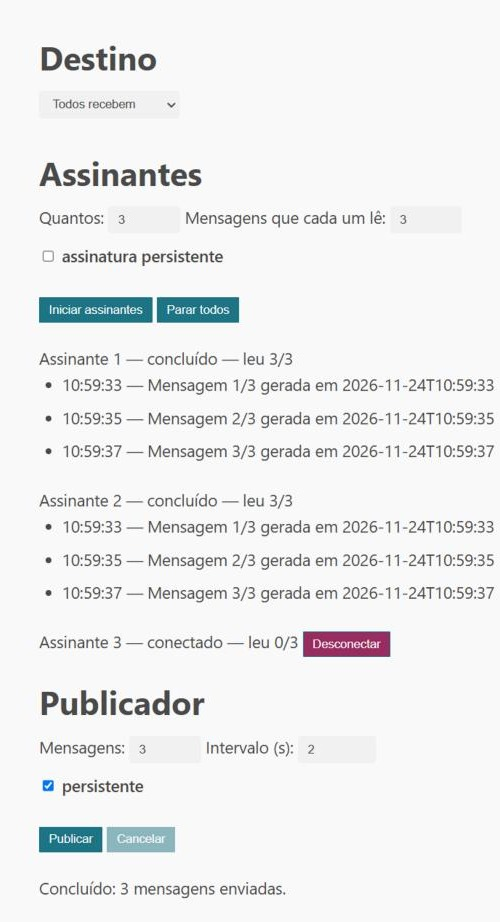
\includegraphics[width=\textwidth]{figuras/php-naoduravel.jpg}
  \caption{T\'opico n\~ao dur\'avel: depois de reconectar, o Assinante~3 continua com 0/3.}
\end{subfigure}
\caption{P\'agina web nos cen\'arios de fila e de t\'opico n\~ao dur\'avel.}
\label{fig:filand}
\end{figure}

\begin{figure}[htbp]
\centering
\begin{subfigure}{0.46\textwidth}
  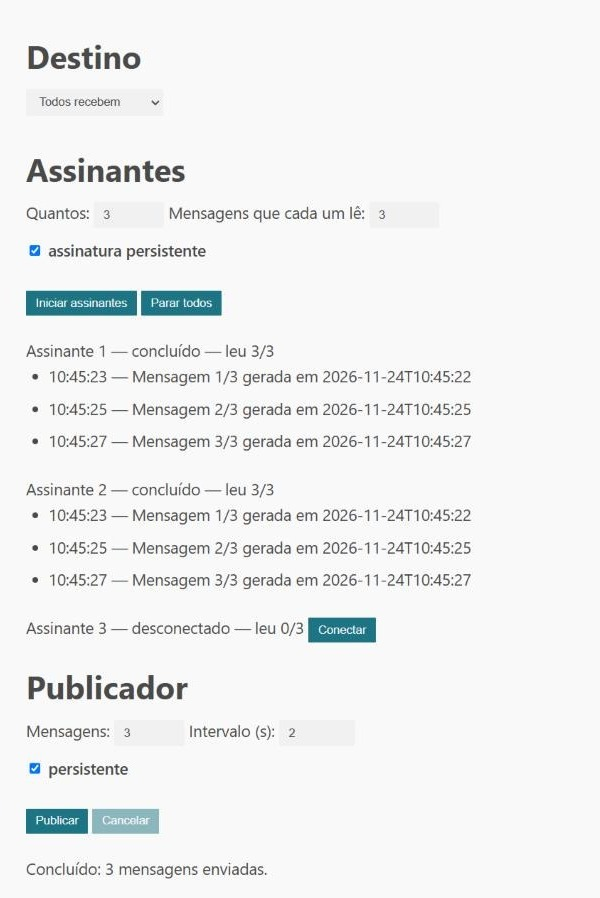
\includegraphics[width=\textwidth]{figuras/php-duravel-offline.jpg}
  \caption{Durante o envio (offline).}
\end{subfigure}\hfill
\begin{subfigure}{0.46\textwidth}
  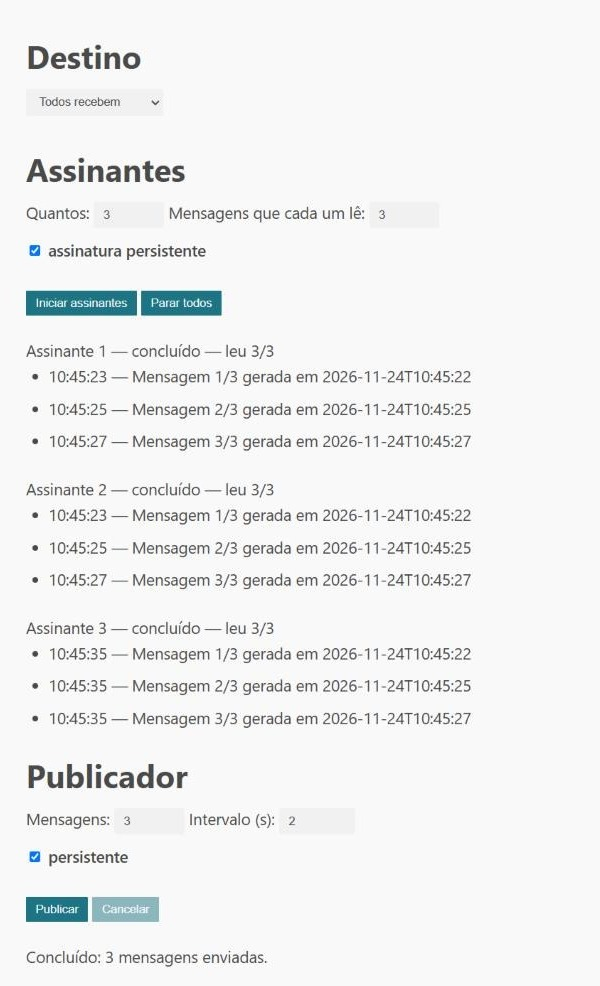
\includegraphics[width=\textwidth]{figuras/php-duravel-reconectado.jpg}
  \caption{Depois de reconectar.}
\end{subfigure}
\caption{Assinatura dur\'avel: o Assinante~3 recebeu as tr\^es mensagens ao voltar.}
\label{fig:dur}
\end{figure}

\logfig{logs/php-terminal-naoduravel.txt}{N\~ao dur\'avel no terminal: o assinante n\~ao recebe nada.}{log:nd}
\logfig{logs/php-terminal-duravel.txt}{Dur\'avel no terminal: a assinatura \'e criada, o assinante sai, as mensagens s\~ao publicadas e depois entregues; no fim a assinatura \'e removida.}{log:dur}

\subsection{Cen\'ario 5: persistente $\times$ n\~ao persistente}
Foram publicadas tr\^es mensagens persistentes numa fila e tr\^es n\~ao persistentes
em outra, sem assinantes. Depois de reiniciar o \textit{broker}
(\texttt{docker restart}), as tr\^es persistentes foram entregues e as n\~ao
persistentes se perderam (Log~\ref{log:pers}).

\logfig{logs/php-terminal-persistencia.txt}{Persist\^encia com reinicializa\c{c}\~ao do \textit{broker}.}{log:pers}

\subsection{Resumo}
\begin{table}[htbp]
\centering
\small
\begin{tabular}{@{}p{5.6cm}p{6.4cm}c@{}}
\toprule
\textbf{Cen\'ario} & \textbf{Resultado esperado} & \textbf{Resultado} \\
\midrule
1. Fan-out (t\'opico)                       & todos recebem a mesma mensagem         & confirmado \\
2. Fila                                     & cada mensagem vai a um s\'o assinante   & confirmado \\
3. T\'opico n\~ao dur\'avel, assinante offline & mensagens perdidas                     & confirmado \\
4. Assinatura dur\'avel, assinante offline    & mensagens entregues na volta           & confirmado \\
5. Persistente $\times$ n\~ao persistente    & s\'o as persistentes sobrevivem ao restart & confirmado \\
\bottomrule
\end{tabular}
\caption{Resultados dos cinco cen\'arios.}
\end{table}

\subsection{Dificuldades}
\begin{itemize}
  \item \textbf{Remo\c{c}\~ao da assinatura dur\'avel.} O \textit{broker} recusa a remo\c{c}\~ao
        enquanto o consumidor est\'a ativo (erro \emph{``Durable consumer is in use''}).
        \'E preciso desligar o consumidor e s\'o ent\~ao enviar o \texttt{UNSUBSCRIBE} com
        o nome da assinatura, o que a biblioteca n\~ao faz sozinha.
  \item \textbf{Assinantes vivos na p\'agina web.} Como cada requisi\c{c}\~ao web termina logo,
        foi preciso iniciar os assinantes como processos em segundo plano, que gravam o
        estado em arquivos lidos pela p\'agina.
  \item \textbf{Redesenho da lista.} Inicialmente o estado enviado \`a p\'agina inclu\'ia um
        hor\'ario que mudava a cada segundo, e a lista de assinantes era redesenhada
        o tempo todo, o que podia fazer um clique se perder. O hor\'ario foi retirado da
        resposta e a lista s\'o muda quando algo muda de verdade.
\end{itemize}

\section{Conclus\~ao}

O laborat\'orio mostrou, na pr\'atica, as diferen\c{c}as entre t\'opico e fila, entre
persist\^encia da mensagem e durabilidade da assinatura, e como o STOMP permite usar um
\textit{broker} de mensagens a partir do PHP com poucos recursos. O publicador enviou as
cinco mensagens com intervalo de um minuto e as cinco inst\^ancias leram uma mensagem
cada: todas a mesma no t\'opico, e uma diferente por inst\^ancia na fila. Os cen\'arios de
assinatura dur\'avel e de persist\^encia tamb\'em se comportaram como a teoria prev\^e.

\begin{thebibliography}{99}\small

\bibitem{savoir} Savoir Technologies.
\newblock \emph{ActiveMQ Essentials -- Queues vs Topics}. V\'ideo.
\newblock \url{https://youtu.be/PtPuR0qcE0c}.

\bibitem{redblack} Red Black Tech.
\newblock \emph{System Design Interview Prep: Queue vs PubSub}. V\'ideo.
\newblock \url{https://youtu.be/ac2zC2YsXnI}.

\end{thebibliography}

\end{document}
